\chapter{Methodology}    

Aim of this project is to classify the vehicles around the host vehicle into normal and abnormal or simply safe or dangerous. For this purpose first step is to identify and classify  the vehicles. After that features of moving vehicles are extracted to classify them into normal and abnormal vehicles. These features are basically motion features i.e. motion vectors of moving vehicles. Basically, we will have to detect vehicles, find the direction, speed i.e. velocity and other properties of the detected vehicles and then classify them into safe or unsafe categories. Figure 3.1 describes an approach, that can be used to solve this problem :

\vspace{10mm}
\begin{figure}[h]
\begin{center}
     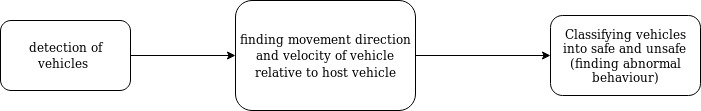
\includegraphics[scale=0.6]{approach.jpg}
    \caption{Steps in proposed method}
\end{center}
   
\end{figure}

\section{Detection of Vehicles}
A fast and accurate object detection system is needed which can work in real time video processing. For this, methods used in previous works like background subtraction methods, filtering etc. or stochastic machine learning methods can not be used because they are slow and less accurate. So to make this object detection faster and accurate  YOLO algorithm \cite{yolo} is used which is best known for its speed in object detection and also it is current state of art for object detection.

YOLO solves the object detection problem as a regression problem instead of a classification problem. It does not need to iterate single image many times but just analyse it only once achieving the speed of up-to 45 fps. It will return center coordinates, height, width of the bounding box which will contain the vehicle.

\section{Motion Analysis of Vehicles}
After the vehicles have been detected and localized, next step is to find the movement direction of vehicles. For this purpose, optical flow analysis is done which will give motion vector for moving objects. There are many methods available for optical flow analysis, but Lucas-Kanade algorithm \cite{lucas} is used in this project. 

The Lucas-Kanade method assumes that the displacement of the image contents between two nearby instants (frames) is small and approximately constant within a neighborhood of the point(which is received from previous step) under consideration. This will return motion vectors for some moving pixels (depends on implementation and arguments passed to Lucas-Kanade algorithm). These multiple motion vectors are aggregated using simple averaging into one motion vector corresponding to each vehicle. Thus at the end of this step, motion information of all the vehicle in current frame is available.

\section{Classification and Finding Abnormal Behaviour}
After calculation of the optical flow vectors(which is w.r.t to the host vehicle) for each the vehicles, some optical flow vectors with  very small magnitude(speed) are eliminated by setting a practical threshold. For the rest of optical flow vectors classification is carried out to identify the abnormal vehicles. A custom trained model is used for this classification task. For this purpose, support vector machine algorithm \cite{svm} is used. After that the vehicles are marked/alarmed as abnormal and normal accordingly.

Following flowchart explains the steps taken in the project with specified algorithms:


\begin{figure}[H]
    \centering
    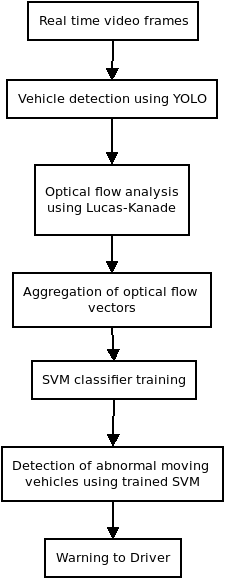
\includegraphics[scale=0.7]{fc.png}
    \caption{Flowchart of the proposed algorithm}
    \label{fig:my_label}
\end{figure}